%!TeX spellcheck = en-US
%!TEX root = ../hw3_report.tex
\subsection*{(a)}
The QR-algorithm is implemented and applied to the given matrix, see Julia code and Figure  \ref{task2}.

\subsection*{(b) and (c)}
The eigenvalues of the matrix A are (by construction) $[2^{[0:7]}, \lambda_9, 2^9]$,
where

\begin{equation}
\lambda_{9} = 2^9\left(0.99-\frac{1}{5\alpha}\right).
\end{equation}
After $n$ iterations, the elements below the diagonal in the QR-iterates will be \emph{proportional} to $|\lambda_i/\lambda_j|^n$, where $i<j$. For large $\alpha$, the dominating eigenvalues are $\lambda_9$ and $\lambda_{10}$. Computing $|\lambda_i/\lambda_j|^n$, for $i = 9$ and $j = 10$, we obtain
\begin{equation}
|\lambda_i/\lambda_j|^n = \left(0.99-\frac{1}{5\alpha}\right)^n.
\end{equation}
Taking this as a measure of the error and setting a tolerance of $10^{-10}$, we obtain
\begin{equation}
\begin{aligned}
\left(0.99-\frac{1}{5\alpha}\right)^n\leq 10^{-10}\\
\Leftrightarrow
n\cdot\log(0.99-\frac{1}{5\alpha})\leq -10 \log(10)\\
n\geq \frac{-10\log(10}{\log(0.99-\frac{1}{5\alpha})}.
\end{aligned}
\end{equation}
The  predicted number of iterations is plotted together with the obtained number of iterations in Figure \ref{task2}. The predicted number of iterations is proportional to the true number of iterations, as expected.

\begin{figure}[h!]
\centering
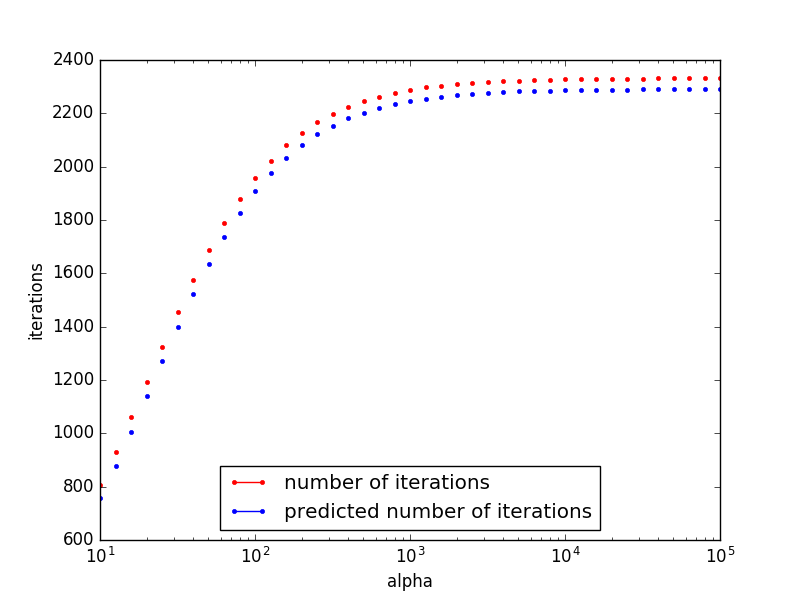
\includegraphics[scale=0.6]{alpha.png}
\caption{Task 2: obtained and predicted number of iterations for the QR-method applied to the given matrix.}
\label{task2}
\end{figure}
